\documentclass[a4paper,12pt]{ctexart}

\usepackage{amsmath}
\usepackage{graphicx}
\usepackage{float}
\usepackage{hyperref}
\usepackage{cite}
\usepackage{algorithm}
\usepackage{algorithmic}

\begin{document}


\section{引言}

伪装目标分析(camouflaged object detection)是对一张图片中的伪装目标进行检测或者分割
,而伪装目标则是指所要分析的目标与背景之间存在颜色、纹理、形状等方面的高度相似性,
这种相似性常见于被捕食者改变它们自身的某些特征,使这些特征与周围环境的特征高度相似,从而躲避捕食者的追击。

而与伪装目标分析相对则是显著目标分析(salient object detection),
显著目标分析所要分析的目标与周围环境在颜色、纹理等特征上存在较大的差异,能够被视觉系统快速、精准的捕捉。
一个典型的例子如图\ref{fig:camouflagedVSSalient}所示。

\begin{figure}[htbp]
    \centering
    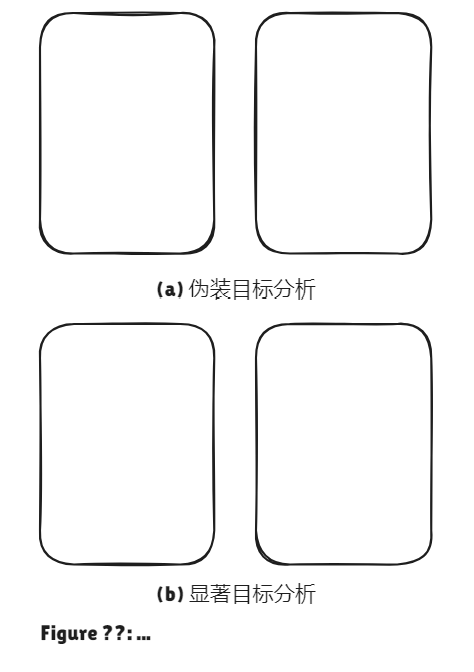
\includegraphics[height=0.5\textheight]{figures/camouflagedVSSalient.png}
    \caption{伪装目标分析与显著目标分析}
    \label{fig:camouflagedVSSalient}
\end{figure}

本报告将围绕伪装目标分割与检测展开,主要使用如下三种方法:
\begin{itemize}
    \item 基于条件随机场(CRF)的伪装目标分割。
    \item 
    \item 
\end{itemize}

\section{相关工作}

\subsection{语义分割}
\textbf{语义分割}是许多视觉理解系统中的核心组成部分,其目的是将图像划分为多个区域。一些早期的方法包括阈值分割\cite{Otsu1979ATS}、基于直方图的分组、区域增长\cite{Nock2004StatisticalRM}、k均值聚类\cite{Dhanachandra2015ImageSU}和分水岭算法\cite{Najman1994WatershedOA}等。这些方法为语义分割奠定了基础,但在复杂场景中往往存在性能限制。近年来,随着深度学习技术的快速发展,语义分割领域迎来了新的变革。深度学习模型通过学习高维特征表示和端到端的优化策略,大幅提升了分割模型的性能。在多个基准数据集上的实验表明,基于深度学习的语义分割方法通常能够取得最高的精度。

\textbf{基于区域分类的语义分割方法} 这一类方法采用自下而上的图像分割方法,生成候选区域后,结合DCNN对分割区域进行分类。例如,在方法\cite{Arbelez2014MultiscaleCG}和\cite{Uijlings2013SelectiveSF}中利用候选边界框和分割区域,将其作为输入提供给DCNN,通过引入形状信息优化分类过程。类似地,\cite{Mostajabi2014FeedforwardSS}采用超像素表示进行区域分割。这些方法能够从高质量的初始分割中受益,但其性能容易受到初始分割的影响,难以实现后续的纠正。

\subsection{伪装目标分割}
\section{方法}

\subsection{基于条件随机场(CRF)的伪装目标分割}

对于任务一,我将采用如下的流程来进行伪装目标分割任务,简要介绍如下:

\begin{enumerate}
    \item \textbf{深度全卷积网络来获取每个像素的初始一元势能(Unary Potential):} 受到DeepLab\cite{Chen2016DeepLabSI}等相关工作的启发,可以利用深度全卷积网络(DCNN)本身对于视觉信息的强大处理能力,直接使用经过预处理的原始图像作为模型输入,来进行一元势能的提取,为后续条件随机场提供一个较好的迭代初始点,详细模型请见。。
    \item \textbf{基于条件随机场(CRF)的后处理逻辑:} 直接使用DCNN的输出作为最终分割掩码可能会导致分割边界粗糙、过多的错误分割区域,分割区域不连续等问题,这些问题出现的根本原因是全卷积网络对于输出像素间的结构关系预测能力较差,而这正是概率图模型所擅长建模的,具体来说,是条件随机场模型(CRF)。条件随机场模型可以基于一些衡量图像像素特征间特定关系的核函数,来对像素类别的可能取值进行更新与约束,从而使预测分割掩码符合一定的结构性,关于条件随机场模型的更多实现细节可以见。。
\end{enumerate}

接下来,我将首先介绍一些关于数据集的观察发现,随后引出基于该发现随使用的全卷积网络的结构,最后介绍条件随机场模型的后处理逻辑

\subsubsection{基于数据集的发现}
用于训练的数据集组成部分如下:

\textbf{CAMO\cite{Le2019AnabranchNF}:} 该数据集中总共有1250张,其中训练集包含1000张图片,测试集250张图片。

\textbf{COD10k\cite{Fan2020CamouflagedOD}: } 该数据集包含5066张伪装目标图片,3000张背景图片,1934张非伪装目标图片。类别划分为5个超类,78个子类,并且对于每一张伪装目标图片都标注有关键特征(如多目标、小目标、有遮盖,形状复杂等)。从图。。和。。可以看出,小目标伪装图片占数据集的绝大部分,这种数据的分布会导致以下问题:
\begin{enumerate}
    \item \textbf{难以分割出较小伪装目标:} 由于伪装目标占整张图片较小的一部分,如图。。(展示一张示例图片),且其与周围环境存在颜色与纹理上的高度相似性,所以模型会非常容易将伪装目标误分类成背景。所以对于小尺度上的特征提取就非常重要。在本次任务中利用DeepLab模型所提出的多尺度图像处理以及空洞金字塔池化(ASPP)技巧来解决数据集中小伪装目标的问题。
	\item \textbf{背景部分的预测会主导模型的训练过程:} 对于包含较小伪装目标的图片的训练来说,由于伪装类别占整张图片的较少部分,所以用于指导模型参数梯度下降的损失值在平均意义上更偏向于使背景图片分类正确,这样在训练损失值上的体现就是在初期会有一个较大的下降,而在后期保持几乎不变,从可视化也可以看出,模型的输出仅有很小一部分像素,或者没有任何像素,分类为伪装目标。对于该问题的处理,我采用的是基于类别的加权损失计算,即针对伪装目标类别给予较高的权重,而对于背景类别则是较低的权重。
\end{enumerate}


\subsubsection{一元势能提取}
在本任务中,使用基于Resnet-101的全卷积神经网络\cite{Chen2016DeepLabSI}作为提取一元势能的模块,具体设计细节如下:

\textbf{空洞卷积的使用:} 在深度卷积神经网络(DCNN)中,标准的下采样操作\cite{Shelhamer2014FullyCN}(例如最大池化或步幅卷积)会导致特征图的空间分辨率显著下降。这种降维虽然增强了不变性,但同时降低了空间定位精度,尤其在语义分割任务中会影响对边界和小目标的捕获。为了解决这一问题,DeepLab模型通过在卷积核之间插入“空洞”(即零值)形成空洞卷积来扩大感受野,同时保持特征图的空间分辨率。这种方法无需增加参数量或计算开销,即可在网络中保留更高的分辨率特征。具体实现中,DeepLab 将 ResNet-101 的最后几层池化操作的步幅设为 1,并使用空洞卷积以确保特征响应的密集性,最后使用双线性插值将特征图恢复到原始图像分辨率


\textbf{多尺度分割的处理:} DeepLab模型通过两种方式来处理多尺度分割:
\begin{enumerate}
    \item \textbf{多尺度输入:} 首先通过将输入图像调整为不同的尺寸(如 0.5x、0.75x、1x),然后分别输入到共享参数的 DCNN 中进行特征提取。最后,通过插值将特征图恢复到原始尺寸并采用最大值融合的方式进行多尺度融合。
    \item \textbf{空洞空间金字塔池化(ASPP):} 该模块包含多个并行的分支,每个分支使用不同的空洞率 $r$ 和固定的卷积核(如 $3 \times 3$)。具体设置包括:总共有四个不同的空洞率,分别是6,12,18,24,小空洞率用于捕获细粒度的特征,大空洞率用于捕获全局上下文信息。
\end{enumerate}

在训练阶段,模型分别输出图像在三个尺度下的响应,以及最大值融合响应用于指导训练过程。在推理阶段,模型只输出最大值融合响应最为预测结果,该响应即为条件随机场的一元势能

\subsubsection{基于全连接条件随机场的后处理逻辑}

在语义分割中,DCNN生成的像素级分类得分图通常是平滑的,但在物体边界处可能会失去细节或出现模糊。为了解决这一问题,可以使用全连接 CRF 模型建模像素间的二元结构关系,增强边界定位并消除伪预测。

\paragraph{能量函数定义}
    全连接 CRF 使用以下能量函数 $E(x)$ 对像素标签分配进行建模:
    $$
    E(x) = \sum_{i} \theta_i(x_i) + \sum_{i,j} \theta_{ij}(x_i, x_j)
    $$
    \begin{itemize}
        \item \textbf{一元势能} $\theta_i(x_i)$:由上述DeepLab的最大值融合响应给出
        \item \textbf{二元势能} $\theta_{ij}(x_i, x_j)$:定义像素 $i$ 和 $j$ 之间的相互作用,旨在通过像素的空间和颜色相似性对分类进行约束。     
    \end{itemize}

\paragraph{二元势能的建模}
    二元势能采用了两种高斯核函数建模像素间关系:
    $$
    \theta_{ij}(x_i, x_j) = \mu(x_i, x_j) \left[ w_1 \exp \left( -\frac{\|p_i - p_j\|^2}{2\sigma_\alpha^2} - \frac{\|I_i - I_j\|^2}{2\sigma_\beta^2} \right) + w_2 \exp \left( -\frac{\|p_i - p_j\|^2}{2\sigma_\gamma^2} \right) \right]
    $$
    \begin{itemize}
    \item 第一项是\textbf{双边核(bilateral kernel)},依赖于像素位置 $p$ 和颜色 $I$,强制空间位置相近且颜色相似的像素拥有相同的标签。
    \item 第二项是\textbf{空间核(spatial kernel)},仅基于像素位置,鼓励空间邻近的像素具有相同标签。
    \item $\mu(x_i, x_j)$ 是 Potts 模型,只有当像素 $x_i \neq x_j$ 时,$\mu(x_i, x_j) = 1$,以确保标签不一致时施加惩罚。
    \end{itemize}

\paragraph{推理}
推理过程采用均值场近似以实现高效的推理,更新算法见\ref{alg:meanfield},更新函数如下:
$$
Q_i(Y_i = l) = \frac{1}{Z_i} \exp \left( -\phi_{u,i}(Y_i) - \sum_{l' = 1}^{L} \mu(l, l') \sum_{k=1}^{K} w_k \sum_{j \neq i} g_k(f_i, f_j) Q_j(l') \right)
$$
\begin{algorithm}
    \caption{均值场近似}
    \label{alg:meanfield}
    \begin{algorithmic}[1]
    \STATE $Q_i(Y_i) \leftarrow \frac{1}{Z_i} \exp\left(-\phi_{u,i}(Y_i = l)\right)$ \COMMENT{初始化}
    \WHILE{未收敛}
        \STATE $\hat{Q}_i^k(Y_i = l) \leftarrow \sum_{j \neq i} g_k(f_i, f_j) Q_j(Y_j = l)$ \COMMENT{消息传递}
        \STATE $\tilde{Q}_i(Y_i = l) \leftarrow \sum_{l' \in \mathcal{L}(l, l')} \sum_{k=1}^{K} w_k \hat{Q}_i^k(l')$ \COMMENT{兼容性变换}
        \STATE $Q_i(Y_i) \leftarrow \exp\left(-\phi_{u,i} - \hat{Q}_i(Y_i)\right)$ \COMMENT{局部更新}
        \STATE $Q_i(Y_i) \leftarrow \frac{1}{Z_i} Q_i(Y_i)$ \COMMENT{归一化}
    \ENDWHILE
    \end{algorithmic}
\end{algorithm}

\paragraph{基于贝叶斯优化的参数搜索}
由于CRF在推理过程中,使用预定义的参数化高斯核函数来进行不同像素特征间结构关系的衡量,所以高斯核函数中参数的的取值对最终的分割结果起到至关重要的作用。故在本节中,讨论使用贝叶斯优化算法对条件随机场模型中参数在其参数空间中进行搜索的问题。
条件随机场模型具有如下参数:
\begin{enumerate}
    \item 空间核函数权重 - \text{POS\_W}
    \item 空间核函数标准差 - \text{POS\_XY\_STD}
    \item 双边核函数权重 - \text{BI\_W}
    \item 双边核函数位置标准差 - \text{BI\_XY\_STD}
    \item 双边核函数颜色标准差 - \text{BI\_RGB\_STD}
\end{enumerate}

针对每个参数设置如下参数空间:

\section{实验}

\subsection{数据集}
\subsection{评价指标}
\subsection{实验配置}
\subsection{实验结果}


\subsection{训练过程曲线}

\section{附录}
\subsection{代码}


\bibliographystyle{plain}
\bibliography{references}

\end{document}